\documentclass{whiteboard}
\begin{document}
\begin{frame}[plain,t]
 \bbcover{Grafos}{Algoritmo de Bellman-Ford}{Prof. Edson Alves}{Faculdade UnB Gama}
\end{frame}

\begin{frame}[plain,t]
\begin{tikzpicture}
\node[draw,opacity=0] at (0, 0) {x};
\node[draw,opacity=0] at (14, 8) {x};
 \node[anchor=west] at (0, 7) { \Large \bbbold{Proponentes} };
\end{tikzpicture}
\end{frame}

\begin{frame}[plain,t]
\begin{tikzpicture}
\node[draw,opacity=0] at (0, 0) {x};
\node[draw,opacity=0] at (14, 8) {x};
 \node[anchor=west] at (0, 7) { \Large \bbbold{Proponentes} };
 \node[anchor=north west] at (0.5, 6) { \includegraphics[scale=0.45]{figs/ford.png} };
 \node[anchor=west] at (4.25, 5.5) { \bbbold{Lester Randolph Ford Jr. } };
 \node[anchor=west] at (4.75, 5.0) { \bbtext{(1956)} };
\end{tikzpicture}
\end{frame}

\begin{frame}[plain,t]
\begin{tikzpicture}
\node[draw,opacity=0] at (0, 0) {x};
\node[draw,opacity=0] at (14, 8) {x};
 \node[anchor=west] at (0, 7) { \Large \bbbold{Proponentes} };
 \node[anchor=north west] at (0.5, 6) { \includegraphics[scale=0.45]{figs/ford.png} };
 \node[anchor=west] at (4.25, 5.5) { \bbbold{Lester Randolph Ford Jr. } };
 \node[anchor=west] at (4.75, 5.0) { \bbtext{(1956)} };
 \node[anchor=north west] at (9, 6) { \includegraphics[scale=0.5]{figs/bellman.jpg} };
 \node[anchor=east] at (9, 2.0) { \bbbold{Richard Ernest Bellman} };
 \node[anchor=east] at (8.5, 1.5) { \bbtext{(1958)} };
\end{tikzpicture}
\end{frame}

\begin{frame}[plain,t]
\begin{tikzpicture}
\node[draw,opacity=0] at (0, 0) {x};
\node[draw,opacity=0] at (14, 8) {x};
 \node[anchor=west] at (0, 6) { \Large \bbbold{Características do algoritmo de Bellman-Ford } };
\end{tikzpicture}
\end{frame}

\begin{frame}[plain,t]
\begin{tikzpicture}
\node[draw,opacity=0] at (0, 0) {x};
\node[draw,opacity=0] at (14, 8) {x};
 \node[anchor=west] at (0, 6) { \Large \bbbold{Características do algoritmo de Bellman-Ford } };
 \node[anchor=west] at (0.5, 5) { $\star$ \bbtext{Computa o caminho mínimo de todos os vértices de $G(V, E)$ a um dado nó $s$} };
\end{tikzpicture}
\end{frame}

\begin{frame}[plain,t]
\begin{tikzpicture}
\node[draw,opacity=0] at (0, 0) {x};
\node[draw,opacity=0] at (14, 8) {x};
 \node[anchor=west] at (0, 6) { \Large \bbbold{Características do algoritmo de Bellman-Ford } };
 \node[anchor=west] at (0.5, 5) { $\star$ \bbtext{Computa o caminho mínimo de todos os vértices de $G(V, E)$ a um dado nó $s$} };
 \node[anchor=west] at (0.5, 4) { $\star$ \bbtext{É capaz de processar arestas negativas} };
\end{tikzpicture}
\end{frame}

\begin{frame}[plain,t]
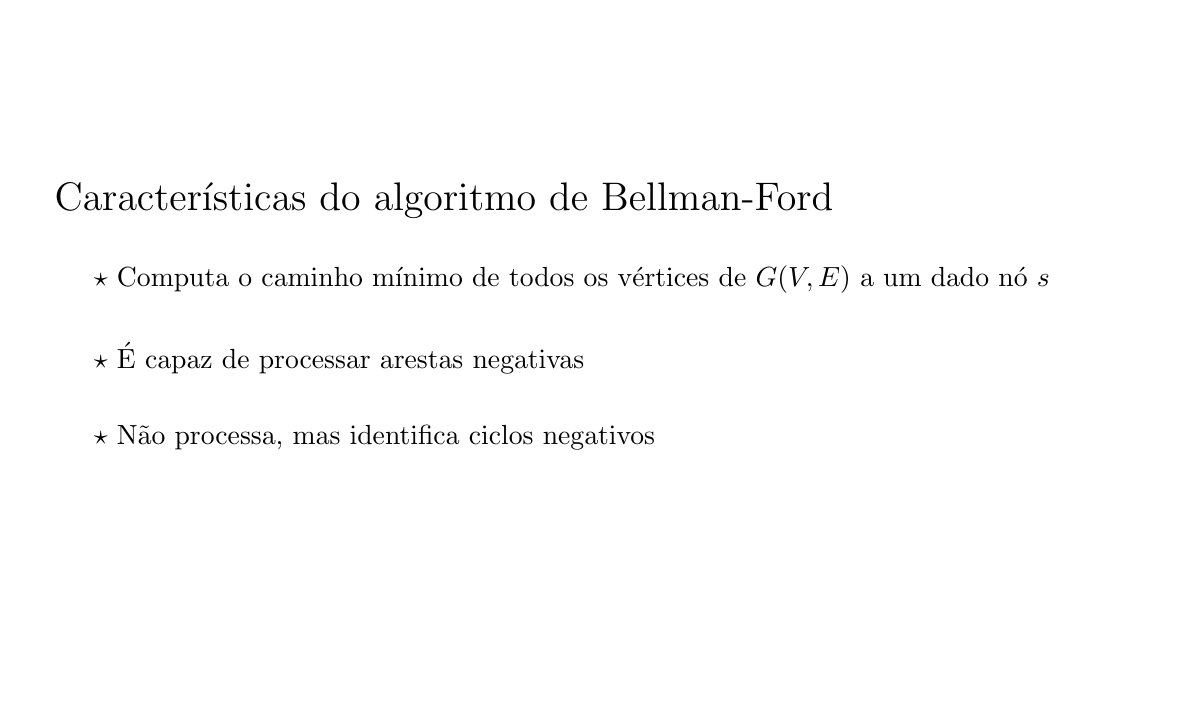
\begin{tikzpicture}
\node[draw,opacity=0] at (0, 0) {x};
\node[draw,opacity=0] at (14, 8) {x};
 \node[anchor=west] at (0, 6) { \Large \bbbold{Características do algoritmo de Bellman-Ford } };
 \node[anchor=west] at (0.5, 5) { $\star$ \bbtext{Computa o caminho mínimo de todos os vértices de $G(V, E)$ a um dado nó $s$} };
 \node[anchor=west] at (0.5, 4) { $\star$ \bbtext{É capaz de processar arestas negativas} };
 \node[anchor=west] at (0.5, 3) { $\star$ \bbtext{Não processa, mas identifica ciclos negativos} };
\end{tikzpicture}
\end{frame}

\begin{frame}[plain,t]
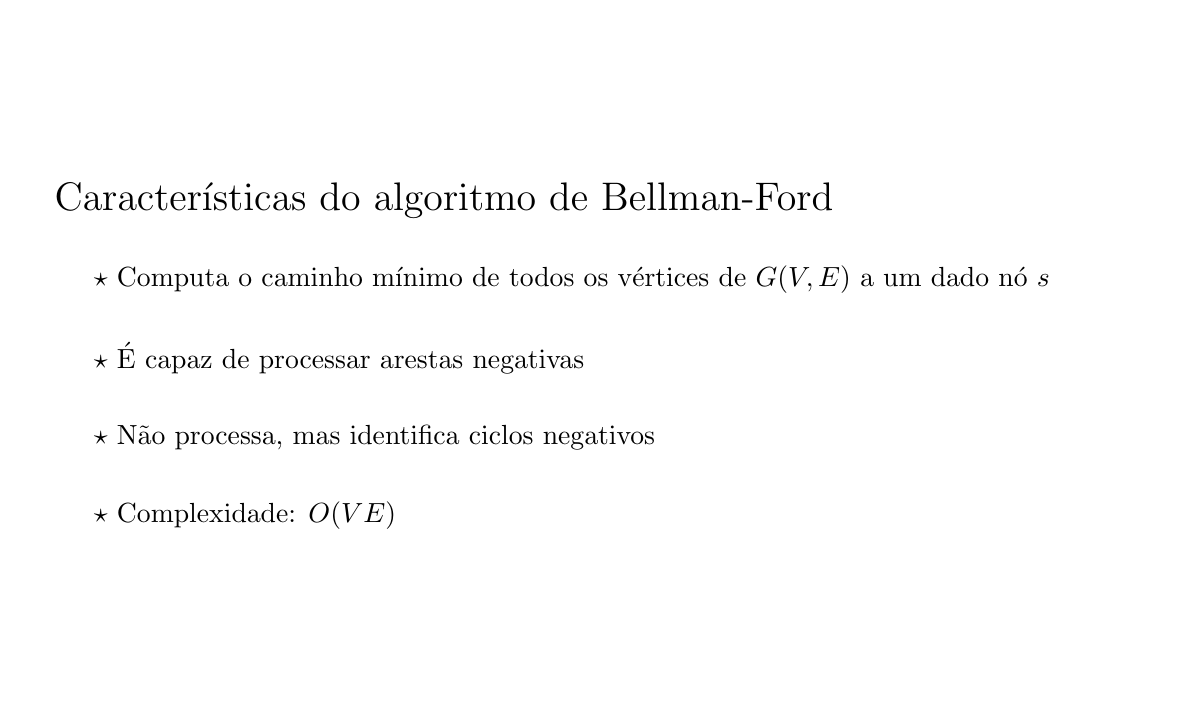
\begin{tikzpicture}
\node[draw,opacity=0] at (0, 0) {x};
\node[draw,opacity=0] at (14, 8) {x};
 \node[anchor=west] at (0, 6) { \Large \bbbold{Características do algoritmo de Bellman-Ford } };
 \node[anchor=west] at (0.5, 5) { $\star$ \bbtext{Computa o caminho mínimo de todos os vértices de $G(V, E)$ a um dado nó $s$} };
 \node[anchor=west] at (0.5, 4) { $\star$ \bbtext{É capaz de processar arestas negativas} };
 \node[anchor=west] at (0.5, 3) { $\star$ \bbtext{Não processa, mas identifica ciclos negativos} };
 \node[anchor=west] at (0.5, 2) { $\star$ \bbtext{\bbbold{Complexidade}: $O(VE)$ } };
\end{tikzpicture}
\end{frame}

\begin{frame}[plain,t]
\begin{tikzpicture}
\node[draw,opacity=0] at (0, 0) {x};
\node[draw,opacity=0] at (14, 8) {x};
 \node[anchor=west] at (0, 7) { \Large \bbbold{Pseudocódigo } };
\end{tikzpicture}
\end{frame}

\begin{frame}[plain,t]
\begin{tikzpicture}
\node[draw,opacity=0] at (0, 0) {x};
\node[draw,opacity=0] at (14, 8) {x};
 \node[anchor=west] at (0, 7) { \Large \bbbold{Pseudocódigo } };
 \node[anchor=west] at (0, 6) { \bbemph{Entrada:} \bbtext{um grafo $G(V, E)$ e um vértice $s\in V$} };
 \node[anchor=west] at (0, 5.5) { \bbemph{Saída:} \bbtext{um vetor $d$ tal que $d[u]$ é a distância mínima em $G$ entre $s$ e $u$ } };
\end{tikzpicture}
\end{frame}

\begin{frame}[plain,t]
\begin{tikzpicture}
\node[draw,opacity=0] at (0, 0) {x};
\node[draw,opacity=0] at (14, 8) {x};
 \node[anchor=west] at (0, 7) { \Large \bbbold{Pseudocódigo } };
 \node[anchor=west] at (0, 6) { \bbemph{Entrada:} \bbtext{um grafo $G(V, E)$ e um vértice $s\in V$} };
 \node[anchor=west] at (0, 5.5) { \bbemph{Saída:} \bbtext{um vetor $d$ tal que $d[u]$ é a distância mínima em $G$ entre $s$ e $u$ } };
 \node[anchor=west] at (1, 4.5) { $1.$ \bbtext{Faça $d[s] = 0$ e $d[u] = \infty$ para todos vértices $u\in V$ tais que $u\neq s$ }};
\end{tikzpicture}
\end{frame}

\begin{frame}[plain,t]
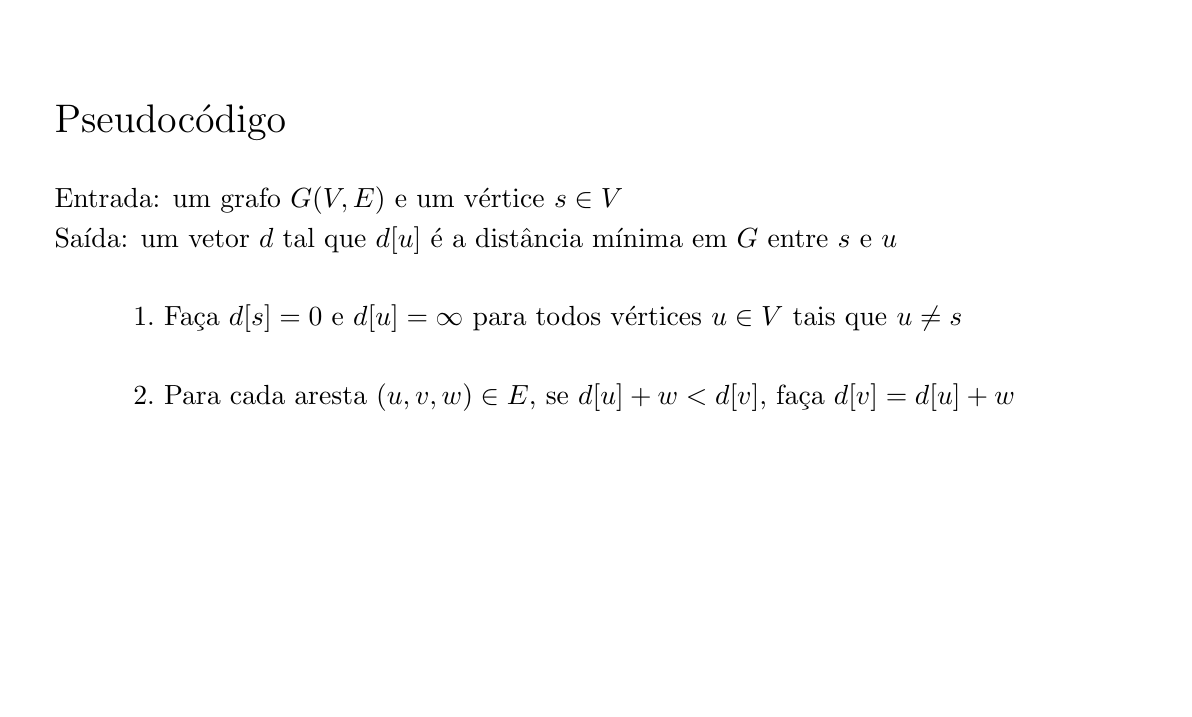
\begin{tikzpicture}
\node[draw,opacity=0] at (0, 0) {x};
\node[draw,opacity=0] at (14, 8) {x};
 \node[anchor=west] at (0, 7) { \Large \bbbold{Pseudocódigo } };
 \node[anchor=west] at (0, 6) { \bbemph{Entrada:} \bbtext{um grafo $G(V, E)$ e um vértice $s\in V$} };
 \node[anchor=west] at (0, 5.5) { \bbemph{Saída:} \bbtext{um vetor $d$ tal que $d[u]$ é a distância mínima em $G$ entre $s$ e $u$ } };
 \node[anchor=west] at (1, 4.5) { $1.$ \bbtext{Faça $d[s] = 0$ e $d[u] = \infty$ para todos vértices $u\in V$ tais que $u\neq s$ }};
 \node[anchor=west] at (1, 3.5) { $2.$ \bbtext{Para cada aresta $(u, v, w)\in E$, se $d[u] + w < d[v]$, faça $d[v] = d[u] + w$} };
\end{tikzpicture}
\end{frame}

\begin{frame}[plain,t]
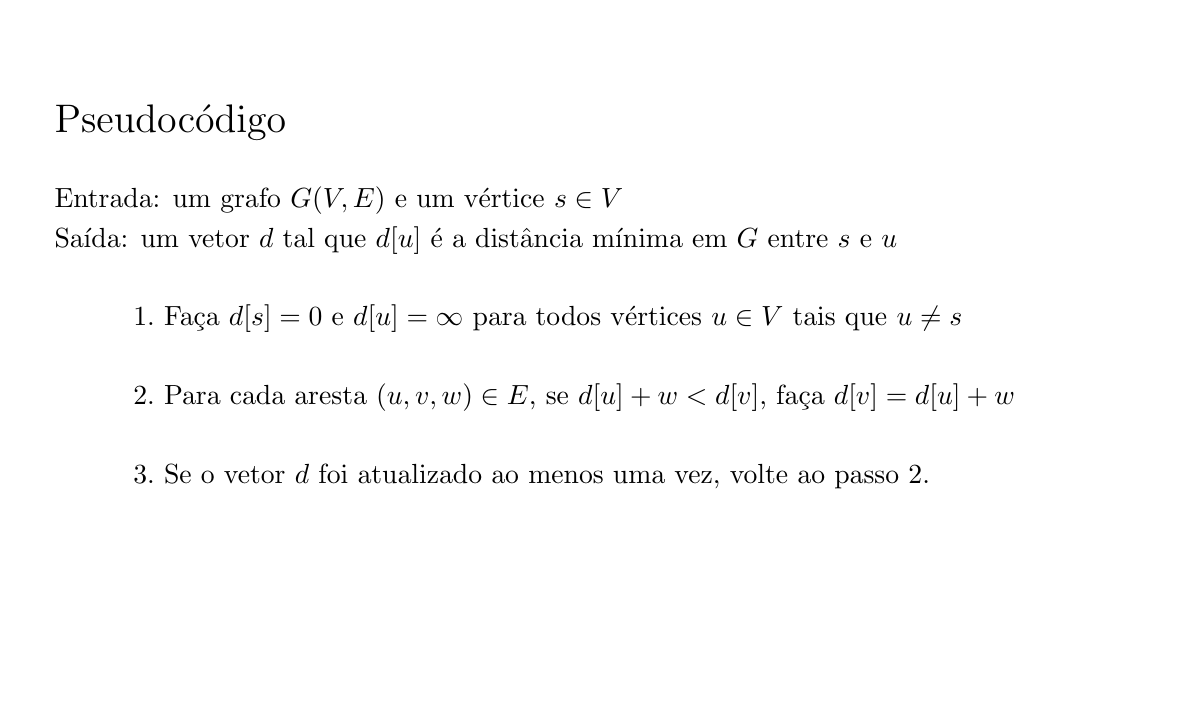
\begin{tikzpicture}
\node[draw,opacity=0] at (0, 0) {x};
\node[draw,opacity=0] at (14, 8) {x};
 \node[anchor=west] at (0, 7) { \Large \bbbold{Pseudocódigo } };
 \node[anchor=west] at (0, 6) { \bbemph{Entrada:} \bbtext{um grafo $G(V, E)$ e um vértice $s\in V$} };
 \node[anchor=west] at (0, 5.5) { \bbemph{Saída:} \bbtext{um vetor $d$ tal que $d[u]$ é a distância mínima em $G$ entre $s$ e $u$ } };
 \node[anchor=west] at (1, 4.5) { $1.$ \bbtext{Faça $d[s] = 0$ e $d[u] = \infty$ para todos vértices $u\in V$ tais que $u\neq s$ }};
 \node[anchor=west] at (1, 3.5) { $2.$ \bbtext{Para cada aresta $(u, v, w)\in E$, se $d[u] + w < d[v]$, faça $d[v] = d[u] + w$} };
 \node[anchor=west] at (1, 2.5) { $3.$ \bbtext{Se o vetor $d$ foi atualizado ao menos uma vez, volte ao passo $2.$ } };
\end{tikzpicture}
\end{frame}

\begin{frame}[plain,t]
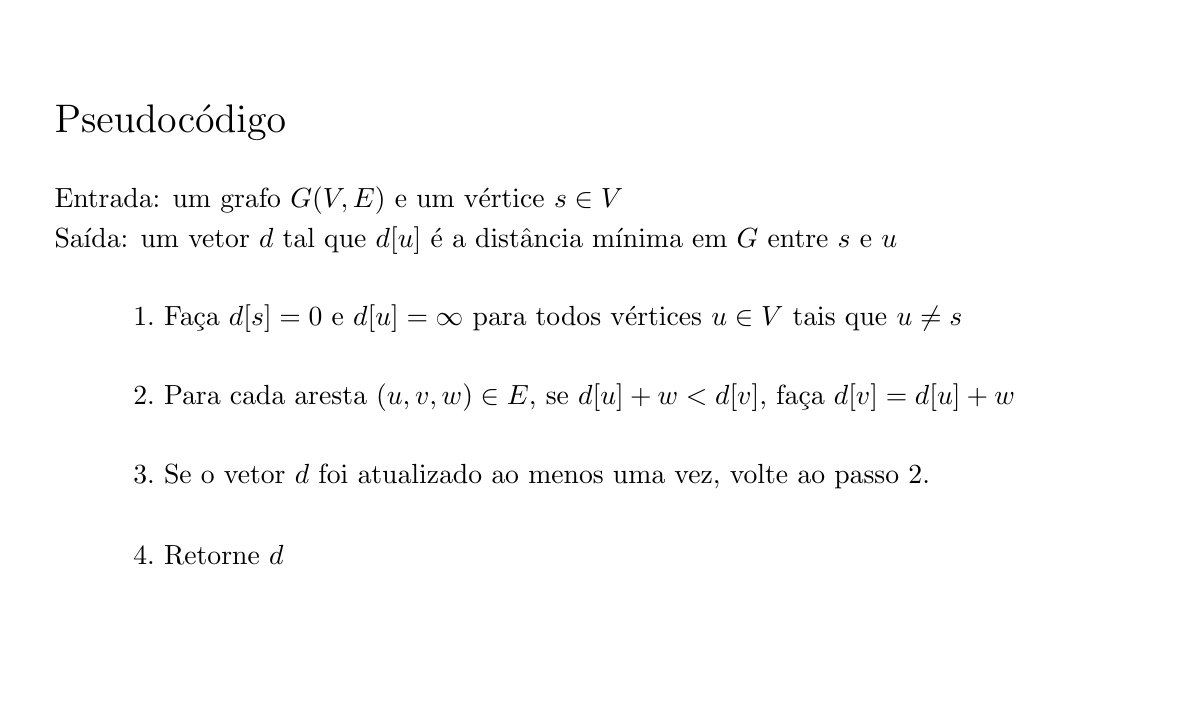
\begin{tikzpicture}
\node[draw,opacity=0] at (0, 0) {x};
\node[draw,opacity=0] at (14, 8) {x};
 \node[anchor=west] at (0, 7) { \Large \bbbold{Pseudocódigo } };
 \node[anchor=west] at (0, 6) { \bbemph{Entrada:} \bbtext{um grafo $G(V, E)$ e um vértice $s\in V$} };
 \node[anchor=west] at (0, 5.5) { \bbemph{Saída:} \bbtext{um vetor $d$ tal que $d[u]$ é a distância mínima em $G$ entre $s$ e $u$ } };
 \node[anchor=west] at (1, 4.5) { $1.$ \bbtext{Faça $d[s] = 0$ e $d[u] = \infty$ para todos vértices $u\in V$ tais que $u\neq s$ }};
 \node[anchor=west] at (1, 3.5) { $2.$ \bbtext{Para cada aresta $(u, v, w)\in E$, se $d[u] + w < d[v]$, faça $d[v] = d[u] + w$} };
 \node[anchor=west] at (1, 2.5) { $3.$ \bbtext{Se o vetor $d$ foi atualizado ao menos uma vez, volte ao passo $2.$ } };
 \node[anchor=west] at (1, 1.5) { $4.$ \bbtext{Retorne $d$ } };
\end{tikzpicture}
\end{frame}

\begin{frame}[plain,t]
\begin{tikzpicture}
\node[draw,opacity=0] at (0, 0) {x};
\node[draw,opacity=0] at (14, 8) {x};
 \node[circle, draw, very thick] (A) at (5, 7.5) { \bbtext{A} };
 \node[circle, draw, very thick] (B) at (2, 5.5) { \bbtext{B} };
 \node[circle, draw, very thick] (C) at (5, 3.5) { \bbtext{C} };
 \node[circle, draw, very thick] (D) at (8, 7.5) { \bbtext{D} };
 \node[circle, draw, very thick] (E) at (11, 5.5) { \bbtext{E} };
 \node[circle, draw, very thick] (F) at (8, 3.5) { \bbtext{F} };
 \draw[thick] (A) to node[above] { \bbinfo{9} } (B);
 \draw[thick] (A) to node[right] { \bbinfo{7} } (C);
 \draw[thick] (A) to node[above] { \bbinfo{4} } (D);
 \draw[thick] (A) to node[below] { \bbinfo{2} } (E);
 \draw[thick] (B) to node[below] { \bbinfo{1} } (C);
 \draw[thick] (B) to node[below,pos=0.8] { \bbinfo{3} } (F);
 \draw[thick] (C) to node[right] { \bbinfo{2} } (D);
 \draw[thick] (D) to node[above] { \bbinfo{1} } (E);
 \draw[thick] (E) to node[below] { \bbinfo{11} } (F);
\end{tikzpicture}
\end{frame}

\begin{frame}[plain,t]
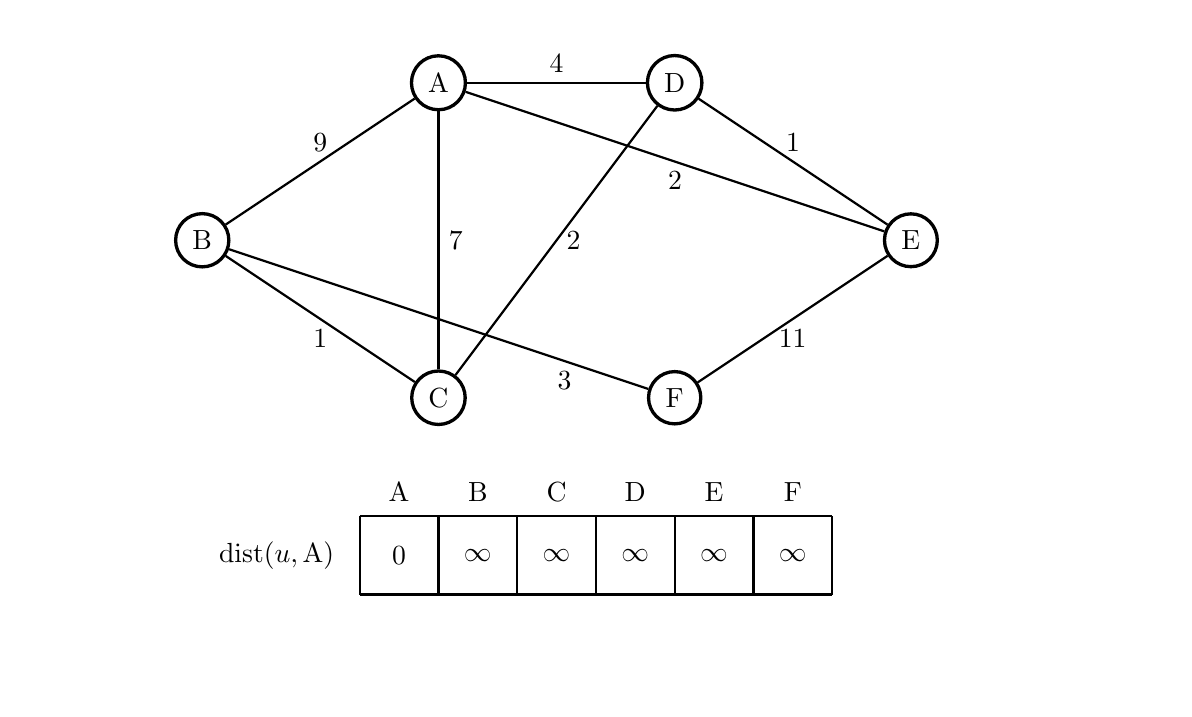
\begin{tikzpicture}
\node[draw,opacity=0] at (0, 0) {x};
\node[draw,opacity=0] at (14, 8) {x};
 \node[circle, draw, very thick] (A) at (5, 7.5) { \bbtext{A} };
 \node[circle, draw, very thick] (B) at (2, 5.5) { \bbtext{B} };
 \node[circle, draw, very thick] (C) at (5, 3.5) { \bbtext{C} };
 \node[circle, draw, very thick] (D) at (8, 7.5) { \bbtext{D} };
 \node[circle, draw, very thick] (E) at (11, 5.5) { \bbtext{E} };
 \node[circle, draw, very thick] (F) at (8, 3.5) { \bbtext{F} };
 \draw[thick] (A) to node[above] { \bbinfo{9} } (B);
 \draw[thick] (A) to node[right] { \bbinfo{7} } (C);
 \draw[thick] (A) to node[above] { \bbinfo{4} } (D);
 \draw[thick] (A) to node[below] { \bbinfo{2} } (E);
 \draw[thick] (B) to node[below] { \bbinfo{1} } (C);
 \draw[thick] (B) to node[below,pos=0.8] { \bbinfo{3} } (F);
 \draw[thick] (C) to node[right] { \bbinfo{2} } (D);
 \draw[thick] (D) to node[above] { \bbinfo{1} } (E);
 \draw[thick] (E) to node[below] { \bbinfo{11} } (F);
 \draw[thick] (4, 1) grid (10, 2);
 \node[anchor=east] at (3.8, 1.5) { $\mathrm{dist}(u, \mbox{\bbtext{A}})$ };
 \node at (4.5, 2.3) { \bbtext{A} };
 \node at (5.5, 2.3) { \bbtext{B} };
 \node at (6.5, 2.3) { \bbtext{C} };
 \node at (7.5, 2.3) { \bbtext{D} };
 \node at (8.5, 2.3) { \bbtext{E} };
 \node at (9.5, 2.3) { \bbtext{F} };
 \node at (4.5, 1.5) { $0$ };
 \node at (5.5, 1.5) { $\infty$ };
 \node at (6.5, 1.5) { $\infty$ };
 \node at (7.5, 1.5) { $\infty$ };
 \node at (8.5, 1.5) { $\infty$ };
 \node at (9.5, 1.5) { $\infty$ };
\end{tikzpicture}
\end{frame}

\begin{frame}[plain,t]
\begin{tikzpicture}
\node[draw,opacity=0] at (0, 0) {x};
\node[draw,opacity=0] at (14, 8) {x};
 \node[circle, draw, very thick] (A) at (5, 7.5) { \bbtext{A} };
 \node[circle, draw, very thick] (B) at (2, 5.5) { \bbtext{B} };
 \node[circle, draw, very thick] (C) at (5, 3.5) { \bbtext{C} };
 \node[circle, draw, very thick] (D) at (8, 7.5) { \bbtext{D} };
 \node[circle, draw, very thick] (E) at (11, 5.5) { \bbtext{E} };
 \node[circle, draw, very thick] (F) at (8, 3.5) { \bbtext{F} };
 \draw[thick] (A) to node[right] { \bbinfo{7} } (C);
 \draw[thick] (A) to node[above] { \bbinfo{4} } (D);
 \draw[thick] (A) to node[below] { \bbinfo{2} } (E);
 \draw[thick] (B) to node[below] { \bbinfo{1} } (C);
 \draw[thick] (B) to node[below,pos=0.8] { \bbinfo{3} } (F);
 \draw[thick] (C) to node[right] { \bbinfo{2} } (D);
 \draw[thick] (D) to node[above] { \bbinfo{1} } (E);
 \draw[thick] (E) to node[below] { \bbinfo{11} } (F);
 \draw[thick] (4, 1) grid (10, 2);
 \node[anchor=east] at (3.8, 1.5) { $\mathrm{dist}(u, \mbox{\bbtext{A}})$ };
 \node at (4.5, 2.3) { \bbtext{A} };
 \node at (5.5, 2.3) { \bbtext{B} };
 \node at (6.5, 2.3) { \bbtext{C} };
 \node at (7.5, 2.3) { \bbtext{D} };
 \node at (8.5, 2.3) { \bbtext{E} };
 \node at (9.5, 2.3) { \bbtext{F} };
 \node at (4.5, 1.5) { $0$ };
 \node at (6.5, 1.5) { $\infty$ };
 \node at (7.5, 1.5) { $\infty$ };
 \node at (8.5, 1.5) { $\infty$ };
 \node at (9.5, 1.5) { $\infty$ };
 \draw[-latex,very thick,color=BBCyan] (A) to node[above] { \bbinfo{9} } (B);
 \node at (5.5, 1.5) { $\mathbf{9}$ };
\end{tikzpicture}
\end{frame}

\begin{frame}[plain,t]
\begin{tikzpicture}
\node[draw,opacity=0] at (0, 0) {x};
\node[draw,opacity=0] at (14, 8) {x};
 \node[circle, draw, very thick] (A) at (5, 7.5) { \bbtext{A} };
 \node[circle, draw, very thick] (B) at (2, 5.5) { \bbtext{B} };
 \node[circle, draw, very thick] (C) at (5, 3.5) { \bbtext{C} };
 \node[circle, draw, very thick] (D) at (8, 7.5) { \bbtext{D} };
 \node[circle, draw, very thick] (E) at (11, 5.5) { \bbtext{E} };
 \node[circle, draw, very thick] (F) at (8, 3.5) { \bbtext{F} };
 \draw[thick] (A) to node[above] { \bbinfo{4} } (D);
 \draw[thick] (A) to node[below] { \bbinfo{2} } (E);
 \draw[thick] (B) to node[below] { \bbinfo{1} } (C);
 \draw[thick] (B) to node[below,pos=0.8] { \bbinfo{3} } (F);
 \draw[thick] (C) to node[right] { \bbinfo{2} } (D);
 \draw[thick] (D) to node[above] { \bbinfo{1} } (E);
 \draw[thick] (E) to node[below] { \bbinfo{11} } (F);
 \draw[thick] (4, 1) grid (10, 2);
 \node[anchor=east] at (3.8, 1.5) { $\mathrm{dist}(u, \mbox{\bbtext{A}})$ };
 \node at (4.5, 2.3) { \bbtext{A} };
 \node at (5.5, 2.3) { \bbtext{B} };
 \node at (6.5, 2.3) { \bbtext{C} };
 \node at (7.5, 2.3) { \bbtext{D} };
 \node at (8.5, 2.3) { \bbtext{E} };
 \node at (9.5, 2.3) { \bbtext{F} };
 \node at (4.5, 1.5) { $0$ };
 \node at (7.5, 1.5) { $\infty$ };
 \node at (8.5, 1.5) { $\infty$ };
 \node at (9.5, 1.5) { $\infty$ };
 \draw[thick] (A) to node[above] { \bbinfo{9} } (B);
 \node at (5.5, 1.5) { $9$ };
 \draw[-latex,very thick,color=BBCyan] (A) to node[right] { \bbinfo{7} } (C);
 \node at (6.5, 1.5) { $\mathbf{7}$ };
\end{tikzpicture}
\end{frame}

\begin{frame}[plain,t]
\begin{tikzpicture}
\node[draw,opacity=0] at (0, 0) {x};
\node[draw,opacity=0] at (14, 8) {x};
 \node[circle, draw, very thick] (A) at (5, 7.5) { \bbtext{A} };
 \node[circle, draw, very thick] (B) at (2, 5.5) { \bbtext{B} };
 \node[circle, draw, very thick] (C) at (5, 3.5) { \bbtext{C} };
 \node[circle, draw, very thick] (D) at (8, 7.5) { \bbtext{D} };
 \node[circle, draw, very thick] (E) at (11, 5.5) { \bbtext{E} };
 \node[circle, draw, very thick] (F) at (8, 3.5) { \bbtext{F} };
 \draw[thick] (A) to node[above] { \bbinfo{4} } (D);
 \draw[thick] (A) to node[below] { \bbinfo{2} } (E);
 \draw[thick] (B) to node[below] { \bbinfo{1} } (C);
 \draw[thick] (B) to node[below,pos=0.8] { \bbinfo{3} } (F);
 \draw[thick] (C) to node[right] { \bbinfo{2} } (D);
 \draw[thick] (D) to node[above] { \bbinfo{1} } (E);
 \draw[thick] (E) to node[below] { \bbinfo{11} } (F);
 \draw[thick] (4, 1) grid (10, 2);
 \node[anchor=east] at (3.8, 1.5) { $\mathrm{dist}(u, \mbox{\bbtext{A}})$ };
 \node at (4.5, 2.3) { \bbtext{A} };
 \node at (5.5, 2.3) { \bbtext{B} };
 \node at (6.5, 2.3) { \bbtext{C} };
 \node at (7.5, 2.3) { \bbtext{D} };
 \node at (8.5, 2.3) { \bbtext{E} };
 \node at (9.5, 2.3) { \bbtext{F} };
 \node at (4.5, 1.5) { $0$ };
 \node at (7.5, 1.5) { $\infty$ };
 \node at (8.5, 1.5) { $\infty$ };
 \node at (9.5, 1.5) { $\infty$ };
 \draw[thick] (A) to node[above] { \bbinfo{9} } (B);
 \node at (5.5, 1.5) { $9$ };
 \draw[-latex,very thick,color=BBCyan] (A) to node[right] { \bbinfo{7} } (C);
 \node at (6.5, 1.5) { $\mathbf{7}$ };
 \draw[thick] (A) to node[above] { \bbinfo{4} } (D);
 \draw[thick] (A) to node[below] { \bbinfo{2} } (E);
 \draw[thick] (B) to node[below] { \bbinfo{1} } (C);
 \draw[thick] (B) to node[below,pos=0.8] { \bbinfo{3} } (F);
 \draw[thick] (C) to node[right] { \bbinfo{2} } (D);
 \draw[thick] (D) to node[above] { \bbinfo{1} } (E);
 \draw[thick] (E) to node[below] { \bbinfo{11} } (F);
\end{tikzpicture}
\end{frame}

\begin{frame}[plain,t]
\begin{tikzpicture}
\node[draw,opacity=0] at (0, 0) {x};
\node[draw,opacity=0] at (14, 8) {x};
 \node[circle, draw, very thick] (A) at (5, 7.5) { \bbtext{A} };
 \node[circle, draw, very thick] (B) at (2, 5.5) { \bbtext{B} };
 \node[circle, draw, very thick] (C) at (5, 3.5) { \bbtext{C} };
 \node[circle, draw, very thick] (D) at (8, 7.5) { \bbtext{D} };
 \node[circle, draw, very thick] (E) at (11, 5.5) { \bbtext{E} };
 \node[circle, draw, very thick] (F) at (8, 3.5) { \bbtext{F} };
 \draw[thick] (A) to node[above] { \bbinfo{4} } (D);
 \draw[thick] (A) to node[below] { \bbinfo{2} } (E);
 \draw[thick] (B) to node[below] { \bbinfo{1} } (C);
 \draw[thick] (B) to node[below,pos=0.8] { \bbinfo{3} } (F);
 \draw[thick] (C) to node[right] { \bbinfo{2} } (D);
 \draw[thick] (D) to node[above] { \bbinfo{1} } (E);
 \draw[thick] (E) to node[below] { \bbinfo{11} } (F);
 \draw[thick] (4, 1) grid (10, 2);
 \node[anchor=east] at (3.8, 1.5) { $\mathrm{dist}(u, \mbox{\bbtext{A}})$ };
 \node at (4.5, 2.3) { \bbtext{A} };
 \node at (5.5, 2.3) { \bbtext{B} };
 \node at (6.5, 2.3) { \bbtext{C} };
 \node at (7.5, 2.3) { \bbtext{D} };
 \node at (8.5, 2.3) { \bbtext{E} };
 \node at (9.5, 2.3) { \bbtext{F} };
 \node at (4.5, 1.5) { $0$ };
 \node at (7.5, 1.5) { $\infty$ };
 \node at (8.5, 1.5) { $\infty$ };
 \node at (9.5, 1.5) { $\infty$ };
 \draw[thick] (A) to node[above] { \bbinfo{9} } (B);
 \node at (5.5, 1.5) { $9$ };
 \draw[-latex,very thick,color=BBCyan] (A) to node[right] { \bbinfo{7} } (C);
 \node at (6.5, 1.5) { $\mathbf{7}$ };
 \draw[thick] (A) to node[above] { \bbinfo{4} } (D);
 \draw[thick] (A) to node[below] { \bbinfo{2} } (E);
 \draw[thick] (B) to node[below] { \bbinfo{1} } (C);
 \draw[thick] (B) to node[below,pos=0.8] { \bbinfo{3} } (F);
 \draw[thick] (C) to node[right] { \bbinfo{2} } (D);
 \draw[thick] (D) to node[above] { \bbinfo{1} } (E);
 \draw[thick] (E) to node[below] { \bbinfo{11} } (F);
\end{tikzpicture}
\end{frame}

\begin{frame}[plain,t]
 \begin{center}\inputsnippet{cpp}{6}{18}{codes/bellman-ford.cpp}\end{center}
\end{frame}

\begin{frame}[plain,t]
\begin{tikzpicture}
\node[draw,opacity=0] at (0, 0) {x};
\node[draw,opacity=0] at (14, 8) {x};
 \node[anchor=west] at (0, 6) { \Large \bbbold{Problemas sugeridos} };
 \node[anchor=west] at (1, 5) { $1.$ \bbtext{AtCoder Beginner Contest 088 -- Problem D: Repainting } };
 \node[anchor=west] at (1, 4) { $2.$ \bbtext{Codeforces Beta Round \#3 -- Problem A: Shortest path of the king } };
 \node[anchor=west] at (1, 3) { $3.$ \bbtext{OJ 10000 -- Longest Paths } };
 \node[anchor=west] at (1, 2) { $4.$ \bbtext{OJ 10959 -- The Party, Part I } };
\end{tikzpicture}
\end{frame}

\begin{frame}[plain,t]
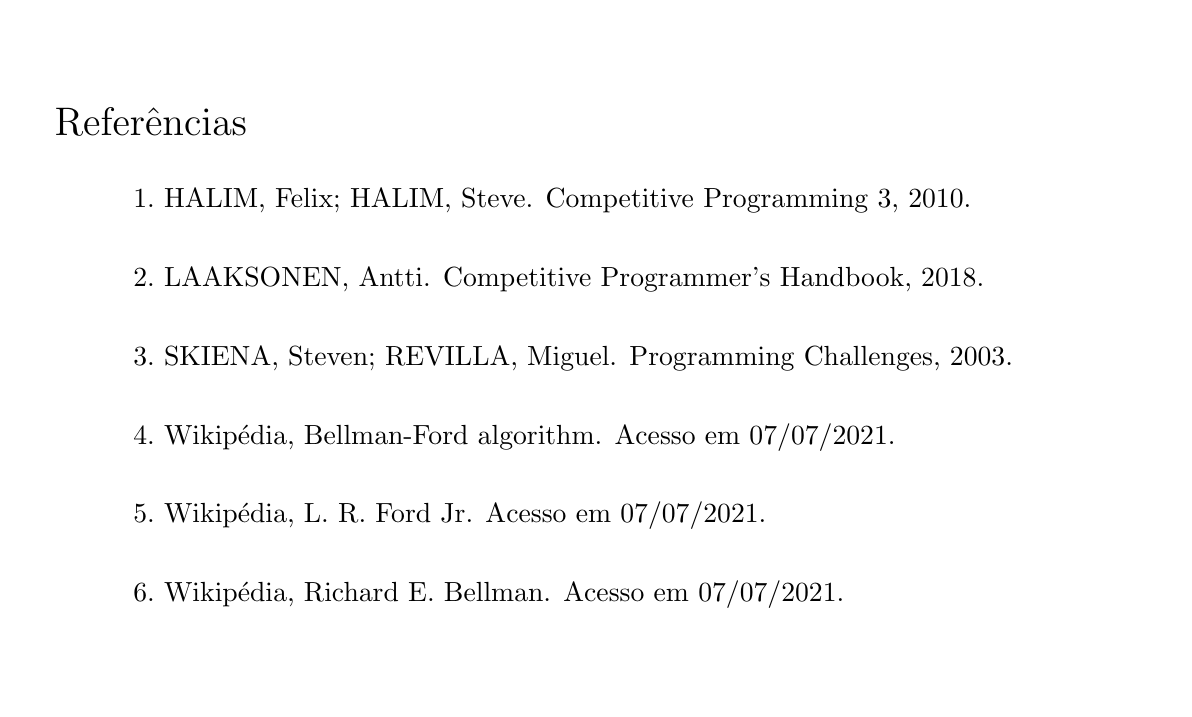
\begin{tikzpicture}
\node[draw,opacity=0] at (0, 0) {x};
\node[draw,opacity=0] at (14, 8) {x};
 \node[anchor=west] at (0, 7) { \Large \bbbold{Referências} };
 \node[anchor=west] at (1, 6) { $1.$ \bbbold{HALIM}, \bbtext{Felix}; \bbbold{HALIM}, \bbtext{Steve}. \bbenglish{Competitive Programming 3,} \bbtext{2010.} };
 \node[anchor=west] at (1, 5) { $2.$ \bbbold{LAAKSONEN}, \bbtext{Antti}. \bbenglish{Competitive Programmer's Handbook,} \bbtext{2018.} };
 \node[anchor=west] at (1, 4) { $3.$ \bbbold{SKIENA}, \bbtext{Steven}; \bbbold{REVILLA}, \bbtext{Miguel}. \bbenglish{Programming Challenges,} \bbtext{2003.} };
 \node[anchor=west] at (1, 3) { $4.$ \bbbold{Wikipédia}, \bbenglish{Bellman-Ford algorithm.} \bbtext{Acesso em 07/07/2021.} };
 \node[anchor=west] at (1, 2) { $5.$ \bbbold{Wikipédia}, \bbenglish{L. R. Ford Jr.} \bbtext{Acesso em 07/07/2021.} };
 \node[anchor=west] at (1, 1) { $6.$ \bbbold{Wikipédia}, \bbenglish{Richard E. Bellman.} \bbtext{Acesso em 07/07/2021.} };
\end{tikzpicture}
\end{frame}

\end{document}
